\chapter{Mushroom}\label{App:msh}
The empirical evaluation of proposed methodologies in \gls{ml} is a critical aspect to take into consideration when publishing a work. Indeed, considering that \gls{ml} is mostly used in practical application, the empirical effectiveness of an algorithm is a desirable property. Because of this reason, the majority of \gls{ml} articles describes a usually extensive empirical section presenting the improvement of the proposed work on the state-of-the-art. This focus on empirical results happens also in \gls{rl} where the algorithms presented in the papers are empirically compared to other methodologies available in literature with the purpose to show some improvements w.r.t. them, e.g. in terms of cumulative discounted reward on several problems.

Several times during my Ph.D. research I needed to implement the code of state-of-the-art algorithms and of the \gls{rl} environments from scratch, since especially at the beginning of my Ph.D. there were not reliable and/or maintained \gls{rl} libraries. Unfortunately, the process of writing codes from scratch for every project was very time consuming and frustrating, especially considering that the same algorithms had to be coded differently just to adapt them to the structure of the ongoing project. Obviously, the problems of time spent in writing code and of reliability of the written code could have been solved with a unified software framework.

For this reason I decided to develop my own \gls{rl} library, which I called \textit{Mushroom}, for helping my research in terms of time and quality. Despite the fact that the development of Mushroom started just for my own purposes, I tried to make it as general as possible and month-by-month it became a general-purpose \gls{rl} library to all effect. Mushroom has the purpose to provide a common interface to develop and run \gls{rl} and it is designed to minimize the effort in writing the code of the experiment: in most cases, the user would only have to write a small script specifying the needed information such as the algorithm to run and the environment. One of the ideas behind Mushroom is to exploit widely used standard libraries such as Pytorch~\cite{paszke2017automatic} and Gym~\cite{gym}, in order to avoid writing new code to implement known algorithms. Mushroom architecture is modular, so that it is possible to include only the needed modules to a system and to implement only the modules that may be needed.

\section{Related works}
Despite the success that \gls{rl} has acquired in the last decade, there are still no standard libraries to perform \gls{rl} experiments. A common interface called RL-Glue~\cite{tanner2009rl} has been proposed in order to allow the communication of agents and environments written in different frameworks and programming languages. However, being only an interface, this library lacks of implementation of \gls{rl} algorithms; furthermore, it is mainly focused on online \gls{rl} algorithms and it is not supported anymore. Nevertheless, a large number of custom libraries are available, but they suffer from heterogeneous drawbacks: poor documentation, lack of algorithms, being very specific for certain tasks or simply no more maintained.

RLPy~\cite{JMLR:v16:geramifard15a} is a good choice to do \gls{rl} experiments with classical algorithms and problems, but currently it does not feature anything related to \gls{drl}; this is an important drawback considering the importance and the ongoing focus of the research on this topic. RLLab~\cite{duan2016benchmarking} is a more modern alternative to RLPy and a good choice for researchers focusing on continuous \gls{drl}. Other recent libraries mostly focused on \gls{drl} However, this library does not cover classical \gls{rl} methodologies and this results in a library useful only for a limited number of researchers. More recent \gls{drl} libraries are TensorForce~\cite{schaarschmidt2017tensorforce} and ChainerRL~\cite{bworld}, that are \gls{rl} extensions of deep learning libraries.

Eventually, there are many libraries featuring a single algorithm. For instance, simple-dqn~\cite{simpledqn} implements the \gls{dqn} algorithm giving the possibility to replicate the experiments in~\cite{mnih2015human} and the low complexity of the code allows to significantly customize it. Of course, the usefulness of such a library is limited to projects related to \gls{dqn}.

\section{Ideas and concepts}
Mushroom is an easily accessible, yet powerful, \gls{rl} library useful for research and didactic purposes.
\paragraph{General purpose} Mushroom adapts to heterogeneous learning tasks based on the interaction of an agent with an environment. This is achieved by a common interface shared by different algorithms, even suitable for different problems: batch and online algorithms, episodic and infinite horizon tasks, on-policy and off-policy learning, and many others.
\paragraph{Lightweight}
Mushroom is both user-friendly and flexible: only a high-level interface is exposed to the user, hiding low-level aspects. For instance, the user should not care about the implementation details to use a function regressor for different tasks, since they are hidden by a simple common interface. However, we leave the check of consistency constraints to the user, e.g. avoiding the use of a tabular algorithm for an environment with continuous state space. Minimal interfaces simplify the implementation of new algorithms, as there are no hard constraints in the prototypes.
\paragraph{Compatible}
Standard Python libraries useful for \gls{rl} tasks have been adopted:
\begin{itemize}
 \item \textit{Scientific calculus}: numpy, scipy;
 \item \textit{Basic \gls{ml}}: scikit-learn;
 \item \textit{\gls{rl} benchmark}: gym;
 \item \textit{Neural networks and \gls{gpu} computation}: pytorch, tensorflow, theano;
 \item \textit{Plotting}: matplotlib.
\end{itemize}
Mushroom provides an interface to these libraries, in order to integrate their functionalities in the framework, e.g. an interface for gym environments, support for regression with scikit-learn models.

\paragraph{Easy to use}
Mushroom enables to develop and run experiments writing a minimal amount of code. In most of the tasks an experiment can be written in a few Python lines without the need of complex configuration files. The majority of the \gls{rl} problems can be solved with experiments written following the structure of the library examples.

\section{Design}
The main module of Mushroom is the \texttt{Core} whose purpose is to manage the interaction between the agent and the environment for both learning and testing tasks.
The common interface \texttt{Environment}, extended by each problem implementation, contains the main properties of the environment: discount factor, horizon (i.e. maximum episode length), observation and action spaces.
Each learning algorithm must extend the \texttt{Agent} class which also provides a common interface to interact with the environment following a specified policy, e.g. a $\varepsilon$-greedy policy.
An instance of the \texttt{Core} class is built providing an agent and an environment object. It defines the \texttt{learn} and the \texttt{evaluate} methods, which implement the interaction of the agent on the environment.

The \texttt{evaluate} method runs the current policy on the environment and collects the dataset. The \texttt{learn} method also feeds the collected dataset to the learning algorithm of the agent, when needed. Both these methods can be run for a fixed number of episodes or steps; moreover, \texttt{learn} allows to specify the frequency, in terms of episodes or steps, of the call to the learning algorithm. Thanks to this choice, it is possible to implement online and batch algorithms transparently. The \texttt{Core} can also run a list of callback functions after each learning step.
\begin{python}
# Online learning running for $30$ episodes
core.learn(n_steps=30, n_steps_per_fit=1)
# Batch learning over a dataset of 30 episodes
core.learn(n_episodes=30, n_episodes_per_fit=30)
# Online learning for 300 episodes, learning every 50 step
core.learn(n_episodes=300, n_steps_per_fit=50)
\end{python}
\begin{figure}[t]
\centering
 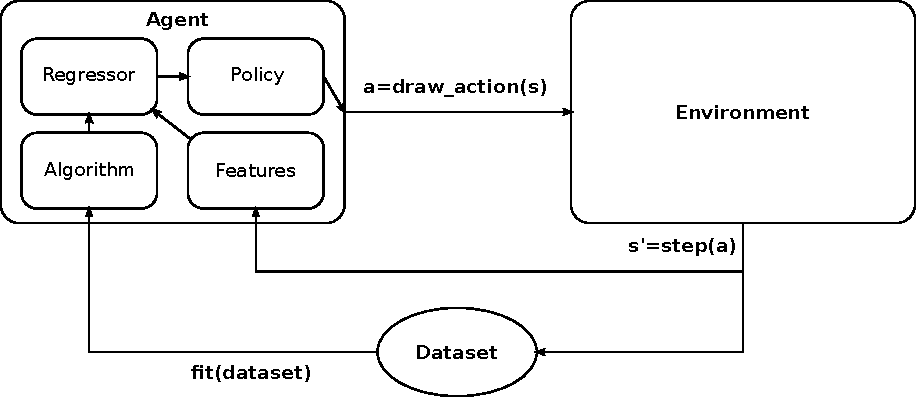
\includegraphics[width=.8\textwidth]{img/msh.pdf}
 \caption[Agent-environment interaction]{Interaction between the agent and the environment when the \texttt{learn} method of the \texttt{Core} class is called. A dataset, collected during this interaction, is used to update the approximator (e.g. policy, $Q$-function).}
\end{figure}\label{F:core}

To simplify the implementation of generic \gls{rl} algorithms, and \gls{td} algorithms in particular, Mushroom offers a high-level interface for the function regressors. This interface supports the use of ensemble regressors that are created specifying the number of models in the ensemble. Moreover, it manages the regressor of the $Q$-function in the case of discrete action spaces: it transparently deals with the creation of a different regressor for each action or a single regressor with a different output for each action. The user should not care about the low-level implementation of these regressors, since everything is managed by the \texttt{Regressor} interface, which also supports generic function approximator. Furthermore, both parametric and non-parametric are transparently managed by the interface.
\begin{python}
# $Q$-function regressor with $5$ different linear approximator
approximator = Regressor(LinearApproximator, n_actions=5, output_shape=(1,), ...)
# $Q$-function regressor with a single linear approximator with 5 outputs
approximator = Regressor(LinearApproximator, n_actions=5, output_shape=(5,), ...)
# Generic linear approximator
approximator = Regressor(LinearApproximator, output_shape=(1,), ...)
\end{python}
The same logic used to implement the \texttt{Regressor} interface, has been used in the \texttt{Features} interface that has the purpose to transparently manage a generic set of basis functions, sparse features (e.g. tiles) and \gls{gpu}-accelerated basis functions implemented with Pytorch~\cite{paszke2017automatic}.
